
\title[概率论]{第一讲:概率论简介}
\author[张鑫 {\rm Email: xzhangseu@seu.edu.cn} ]{\large 张 鑫}
\institute[东南大学数学学院]{\large \textrm{Email: xzhangseu@seu.edu.cn} \\ \quad  \\
  \large 东南大学\quad 数学学院\\
  \vspace{0.3cm}
 % \trc{ 公共邮箱: \textrm{zy.prob@qq.com}\\
  %  \hspace{-1.7cm}  密\qquad 码: \textrm{seu!prob}}
}
%\date{\rm \today}
\date{}


{ \setbeamertemplate{footline}{}
  \begin{frame}
    \titlepage
  \end{frame}
}



\section{ 课程简介}
\subsection{课程说明}
\begin{frame}
	\frametitle{参考书目}
	\begin{itemize}[<+-|alert@+>]
		\item 概率论, 张颢, 高等教育出版社
	    \item 概率论(第二版), 杨振明, 科学出版社
	    \item 概率论基础, 李贤平, 高等教育出版社
	    %\item 概率论基础及其应用, 王梓坤, 北京师范大学出版社
		\item 概率论(第三版), 苏淳,冯群强, 科学出版社
		\item 概率论导论(翻译版), {\rm Joseph K. Blitzstein, Jessica Hwang}\\
	    (张景肖 译), 机械工业出版社
		\item 概率导论(第二版), {\rm Dimitri P. Bertsekas, John N. Tsitsiklis}\\  (郑忠国,童行伟译), 人民邮电出版社
		\item {\rm Probability, A. N. Shiryaev, Springer}
		\item 科学发现纵横谈, 王梓坤, 北京师范大学出版社
	\end{itemize}
\end{frame}




\begin{frame}{参考教材封面}
	\vspace{-0.3cm}
	\begin{columns}
   \column{3cm}
	  \begin{figure}[htbp]\nonumber
		 \centering
		 \includegraphics<+->[width=3cm, height=3.9cm]{prob-zhanghao.jpg}
		 %\caption{约翰·克利斯朵夫(傅雷译)}
		 % \centering{\small 约翰·克利斯朵夫}
	   \end{figure}
	  \column{3cm}
	 \begin{figure}[htbp]\nonumber
		 \centering
		  \includegraphics<+->[width=3cm, height=3.9cm]{prob-yangzhenming.jpg}
		 % \caption{}
		 %  \onslide<2->\centering{\small 肖申克的救赎 }
	   \end{figure}

	   \column{3cm}
	  \begin{figure}[htbp]\nonumber
		 \centering
		 \includegraphics<+->[width=3cm, height=3.9cm]{prob-lixianping.jpg}
		 % \caption{}
		 %  \onslide<3->\centering{\small 闻香识女人 }
	   \end{figure}

	   \column{3cm}
	\begin{figure}[htbp]\nonumber
		 \centering
		 \includegraphics<+->[width=3cm, height=3.9cm]{prob-sucun.jpg}
		 % \caption{}
   %\onslide<4->\centering{\small 心灵捕手 }
	   \end{figure}
	 \end{columns}
\vspace{-0.15cm}
	 \begin{columns}
		\column{3cm}
		   \begin{figure}[htbp]\nonumber
			  \centering
			  \includegraphics<+->[width=3cm, height=3.9cm]{prob-joseph.jpg}
			  %\caption{约翰·克利斯朵夫(傅雷译)}
			   %\centering{\small 约翰·克利斯朵夫}
			\end{figure}
		   \column{3cm}
		  \begin{figure}[htbp]\nonumber
			  \centering
			   \includegraphics<+->[width=3cm, height=3.9cm]{prob-dimi.jpg}
			  % \caption{}
				%\onslide<2->\centering{\small 肖申克的救赎 }
			\end{figure}

			\column{3cm}
		   \begin{figure}[htbp]\nonumber
			  \centering
			  \includegraphics<+->[width=3cm, height=3.9cm]{prob-shiryaev.jpg}
			  % \caption{}
				%\onslide<3->\centering{\small 闻香识女人 }
			\end{figure}

			\column{3cm}
		 \begin{figure}[htbp]\nonumber
			  \centering
			  \includegraphics<+->[width=3cm, height=3.9cm]{prob-wangzikun.jpg}
			  % \caption{}
		%\onslide<4->\centering{\small 心灵捕手 }
			\end{figure}
		  \end{columns}
   \end{frame}


\begin{frame}
	\frametitle{成绩构成}
	\begin{itemize}[<+-|alert@+>]
		\item {\rm  \textcolor{cyan}{20\% - 30\%}} :平时成绩,含平时作业、大作业、讨论报告等。
		%\item  {\rm  \textcolor{cyan}{10\% - 15\%}} : 大作业、课堂讨论报告等
		\item  {\rm  \textcolor{cyan}{20\% - 30\%}}  : 期中随堂测验
		\item  {\rm  \textcolor{cyan}{50\% - 60\%}} : 期末考试
		\item \textcolor{cyan}{5 分}: 课堂及平时表现加分项
		\item 考勤: 不定时随机点名, 如被点到未来上课者每次\textcolor{red}{\bf 扣总评成绩5分}
		\item 期末考试过后, 凡与考试成绩有关的邮件,QQ留言,微信留言均不回复,敬请谅解
	\end{itemize}
\end{frame}

\begin{frame}
	\frametitle{答疑时间与课程{\rm QQ}群}
	\begin{itemize}[<+-|alert@+>]
		\item 答疑
		\begin{itemize}[<+-|alert@+>]
			\item 时间:每周二中午 12:00-13:30
			\item 地点:新文科楼 528-4 办公室
		\end{itemize}
		\item 课程{\rm QQ}群
		\begin{itemize}[<+-|alert@+>]
			\item 理科试验班:814238326
			\item 强基拔尖班:964600973
			\end{itemize}
	\end{itemize}
\end{frame}





\begin{frame}[fragile]
	\frametitle{作业提交}

	\begin{itemize}[<+-|alert@+>]
		\item 自由组合,每两人一组并确定组长由组长提交每次作业
		\item 提交方式:{\rm Gitee}线上提交(Markdown文件与导出的pdf文件)
		\item 提交时间:每周日晚 12 点之前
		\item 如何提交:
		\begin{itemize}[<+-|alert@+>]
			\item 注册Gitee账号并更新个人信息为"学号-姓名":

			强基拔尖班: \href{https://gitee.com/xzhangseu?invite=af354f3608acbf325025111fe2cff3f3d89578f19ae0ba8d8e7cde0b62298f8990135fca197ee75c6b17c049295f276a189625f3b98043645f2e7eaaa8122746}{强基拔尖班邀请链接}%(QQ 群或微信群发送)
			注册 {\rm Gitee}账号.




			理科试验班: \href{https://gitee.com/xzhangseu?invite=af354f3608acbf325025111fe2cff3f3082ca2eb393e34e88e7cde0b62298f8990135fca197ee75c6b17c049295f276a61d258ce9546aa1d5f2e7eaaa8122746}{理科试验班邀请链接}%(QQ 群或微信群发送)
			注册 {\rm Gitee}账号.
			\item  苹果系统已预装{\rm Git}, {\rm Window}系统需下载安装{\rm Git}:

			下载地址:https://git-scm.com/download/ %课程作业仓库至本人{\rm Gitee}账户
			\item \href{https://help.gitee.com/base/account/SSH%E5%85%AC%E9%92%A5%E8%AE%BE%E7%BD%AE}{设置Gitee SSH公钥}, 以便推拉作业仓库

\end{itemize}

	\end{itemize}

\end{frame}

\begin{frame}{Gitee SSH公钥设置}
	\vspace{-0.2cm}
	\begin{columns}
		\column{6cm}
		\begin{figure}[htbp]\nonumber
		\centering
		\includegraphics<+->[width=6cm, height=8cm]{ssh1.png}
		% \caption{}
  %\onslide<4->\centering{\small 心灵捕手 }
	  \end{figure}
	  \column{6cm}

	  \begin{figure}[htbp]\nonumber
		\centering
		\includegraphics<+->[width=6cm, height=6cm]{ssh2.png}
		% \caption{}

	  \end{figure}

	\end{columns}
\end{frame}





\begin{frame}[fragile]{作业提交: Git 命令首次作业提交}

\begin{enumerate}[<+-|alert@+>]
	\item Clone 作业仓库

			强基拔尖班: git clone git@gitee.com:xzhangseu/a-prob-2024.git

			理科试验班: git clone git@gitee.com:xzhangseu/b-prob-2024.git

	\item 创建创建以个人学号-姓名分支:

			git checkout -b 12345-姓名

	\item 将个人新建的分支推送至远程:

			git push {-}{-}set-upstream origin 12345-姓名

	\item 书写作业并提交:

	      git add 作业文件名

		  git commit -m "第k次作业"

		  git push


\end{enumerate}


\end{frame}





\begin{frame}[fragile]{作业提交: Git 命令后续作业提交}

	\begin{enumerate}[<+-|alert@+>]
		\item 更改本地分支到master并拉取作业:

				git checkout master

				git pull

		\item 拉取作业后更改至分支"12345-姓名"完成作业并提交:

				git checkout 12345-姓名

		\item 书写作业并提交:

			  git add 作业文件名

			  git commit -m "第k次作业"

			  git push



	\end{enumerate}
\end{frame}

\begin{frame}{作业格式要求}
\begin{itemize}[<+-|alert@+>]
	\item 作业文件命名为: 第$k$次作业
	\item 作业不能仅有公式,没有语言表达
	\item 作业内容: 标题要添加"第$k$次作业$+$每组两人的学号与姓名", 如下图所示
\end{itemize}

	\begin{figure}[htbp]\nonumber
		\centering
		\includegraphics<+->[width=9.19cm, height=3cm]{homework.jpg}
		% \caption{}
  %\onslide<4->\centering{\small 心灵捕手 }
	  \end{figure}
\end{frame}





\begin{frame}[fragile]{作业提交}
	\begin{itemize}[<+-|alert@+>]
		\item 完成作业需要学习
		\begin{itemize}[<+-|alert@+>]
			\item \href{https://gitee.com/all-about-git}{{\rm Git}知识}
			\item \href{https://gitee.com/oschina/education}{{\rm Gitee}使用}
			\item \href{https://www.markdown.xyz/}{{\rm Markdown}指南}
			\item \href{https://shd101wyy.github.io/markdown-preview-enhanced/\#/zh-cn/}{{\rm Markdown Preview Enhanced}使用指南}
		\end{itemize}
	\end{itemize}
% \begin{lstlisting}[language=Python]
% def main():
% print("Hello, world!")
% return 0
% \end{lstlisting}


\end{frame}





\begin{frame}
	\frametitle{{\rm Markdown}文档编辑软件及插件}
	\begin{itemize}[<+-|alert@+>]
			\item \href{https://code.visualstudio.com/}{\rm Visual Studio Code} 插件
		{\rm 	\begin{itemize}[<+-|alert@+>]
			\item \href{https://shd101wyy.github.io/markdown-preview-enhanced/\#/zh-cn/}{Markdown Preview Enhanced}
            \item \href{https://marketplace.visualstudio.com/items?itemName=OrangeX4.better-markdown-latex-shortcuts}{Better Markdown \& Latex Shortcuts}
            \item \href{https://marketplace.visualstudio.com/items?itemName=hnw.vscode-auto-open-markdown-preview}{Auto-Open Markdown Preview}
            \item \href{https://marketplace.visualstudio.com/items?itemName=bierner.markdown-preview-github-styles}{Markdown Preview Github Styling}
	       \end{itemize}}
            \item \href{https://obsidian.md/}{\rm Obsidian} 插件
           \begin{itemize}[<+-|alert@+>]
			\item  \rm obsidian-latex-suite
			\item  \rm obsidian-latex
			\item  \rm math-booster
			\item  \rm dataview
			\item  \rm mathlinks
	       \end{itemize}
       \item \href{https://logseq.com/}{\rm logseq}
	\end{itemize}
\end{frame}

\begin{frame}
	\frametitle{一些期望}
	\begin{itemize}[<+-|alert@+>]
		\item 守时:作业按规定时间提交
		\item  勇于表现,不做沉默者
		\item  培养批判性思维
		\item 相互尊重,教学意见及时与老师沟通
		\item 注重培养书面语言表达能力
		\item 实事求是、客观的进行教学评价
		%\item 与数学分析的相关内容类比
	\end{itemize}
\end{frame}

\begin{frame}
	\frametitle{学习方法}
	\begin{itemize}[<+-|alert@+>]
		\item 课前预习
		\item 课上学习
		\item 课后复习
		\item 每2-3周完整复习前2-3周的学习内容
		%\item 与数学分析的相关内容类比
	\end{itemize}
\end{frame}

% \begin{frame}
% 	\frametitle{一本书三部电影}
% 	\begin{itemize}[<+-|alert@+>]
% 		\item  约翰·克利斯朵夫(傅雷译)%:面对苦难,何以自处
% 		\item 肖申克的救赎({\rm The Shawshank Redemption})%:毅力,责任,改变世界
% 		\item  闻香识女人({\rm Scent of a Woman})%:%面对诱惑,原则与底线
% 		\item 心灵捕手({\rm  Good Will Hunting})%: 追随内心,

% 		%\item 与数学分析的相关内容类比
% 	\end{itemize}
% \end{frame}




%\begin{frame}{一本书三部电影}
%\begin{columns}
%	\begin{column}{.25\textwidth}
%		\includegraphics<+->[width=3cm, height=4.5cm]{yh.jpg}
%		%\caption{约翰·克利斯朵夫(傅雷译)}
%		\centering{\small 约翰·克利斯朵夫}
%	\end{column}
%
%	\begin{column}{.25\textwidth}
%		\includegraphics<+->[width=3cm, height=4.5cm]{tsr.jpg}
%		% \caption{}
%		\onslide<2->\centering{\small 肖申克的救赎 }
%	\end{column}
%
%	\begin{column}{.25\textwidth}
%		\includegraphics<+->[width=3cm, height=4.5cm]{sm.jpg}
%		% \caption{}
%		\onslide<3->\centering{\small 闻香识女人 }
%	\end{column}
%	\begin{column}{.25\textwidth}
%		\includegraphics<+->[width=3cm, height=4.5cm]{gh.jpg}
%		% \caption{}
%		\onslide<4->\centering{\small 心灵捕手 }
%	\end{column}
%\end{columns}
%\end{frame}


\begin{frame}{一本书三部电影}
 \begin{columns}
\column{3cm}
   \begin{figure}[htbp]\nonumber
      \centering
      \includegraphics<+->[width=3cm, height=4.5cm]{yh.jpg}
      %\caption{约翰·克利斯朵夫(傅雷译)}
       \centering{\small 约翰·克利斯朵夫}
    \end{figure}
   \column{3cm}
  \begin{figure}[htbp]\nonumber
      \centering
       \includegraphics<+->[width=3cm, height=4.5cm]{tsr.jpg}
      % \caption{}
		\onslide<2->\centering{\small 肖申克的救赎 }
    \end{figure}

    \column{3cm}
   \begin{figure}[htbp]\nonumber
      \centering
      \includegraphics<+->[width=3cm, height=4.5cm]{sm.jpg}
      % \caption{}
		\onslide<3->\centering{\small 闻香识女人 }
    \end{figure}

    \column{3cm}
 \begin{figure}[htbp]\nonumber
      \centering
      \includegraphics<+->[width=3cm, height=4.5cm]{gh.jpg}
      % \caption{}
\onslide<4->\centering{\small 心灵捕手 }
    \end{figure}
  \end{columns}


\end{frame}




%\begin{frame}
%	\frametitle{成绩构成}
%	% \frametitle{教材、成绩、学习}
%%	\begin{itemize}[<+-|alert@+>]
	%%		\item 10\% :平时作业成绩
	%%		\item 10\% : 大作业、课堂讨论报告
	%%		\item 20\% : 随堂测验
	%%		\item 60\% : 期末考试
	%%		\item 5 分: 课堂提问回答加分项
	%%	\end{itemize}
%\end{frame}

%\begin{frame}
%	\frametitle{学习方法」
	%%		\begin{itemize}[<+-|alert@+>]
		%%			\item 课前预习
		%%
		%%			\item 课上听课
		%%
		%%			\item 课后复习
		%%
		%%			\item 与数学分析的相关内容类比
		%%
		%%		\end{itemize}
	%	\end{frame}
\subsection{为什么要学概率论?}

\begin{frame}
	\frametitle{什么是概率}


		\begin{itemize}[<+-|alert@+>]
			\item 运气、巧合、随机性、不确定性、风险、时运、机会 - 用法模糊
			\item 概率普遍存在于科学与日常生活中,但可能非常反直觉
			\item 单纯依靠直觉,会出现预测不准确或面临预测过于自信带来严重风险
			\item 概率论课程旨在搭建一个有原则的量化不确定性和随机性的逻辑框架,通过学习强化自身的直觉
		\end{itemize}




\end{frame}





\begin{frame}
	\frametitle{几个问题}
	\begin{prob}
		假设对于概率论课程成绩有两种不同的方式确定, 你选择哪一种?
		\begin{itemize}[<+-|alert@+>]
			\item 课程成绩由提交作业的次数来决定,只要至少提交过 6 次作业就给你 60 分;
			\item 课程成绩由某随机试验的结果来决定,但我保证: 你的课程成绩小于 60 分的概率为 0.
		\end{itemize}

	\end{prob}


\end{frame}


\begin{frame}
	\frametitle{几个问题}

	\begin{prob} 某人医院体检报告甲胎蛋白({\rm AFP})值偏高, 医生建议进行肝细胞活检, 当问及原因时,医生说: 我们发现在肝癌患者中, 有 99.9\% 的患者其甲胎蛋白数值都偏高.  医生给出活检的理由是否充分?
	\end{prob}
\end{frame}

% \begin{frame}
	%   \frametitle{几个问题}
	%   \begin{prob} 某人医院体检报告甲胎蛋白(AFP)值偏高, 医生建议进行肝细胞活检, 当问及原因时,医生说: 我们发现在肝癌患者中, 有 99.9\% 的患者其甲胎蛋白数值都偏高.  医生给出活检的理由是否充分?
		%   \end{prob}
	% \end{frame}

\begin{frame}
	\frametitle{几个问题}
	\begin{prob}三门问题: 在某电视节目中,主持人蒙提霍尔会选择一名观众参与一个游戏.
		\begin{itemize}[<+-|alert@+>]
			\item 三扇门: 一扇门后是一辆汽车, 另外两扇门后各有一只山羊;
			\item 参与者可从三扇门中任选一扇,并可以获得该扇门后的奖品;
			\item 在揭晓参与者所选门后的奖品之前, 主持人会打开其中一个未被选中的一扇门,并揭晓门后的奖品是山羊.

			\item 参与者可以坚持原来的选择或换成剩下的那扇门;
			\item  \textcolor{cyan}{问题}: 参与者是否要改变自己的选择?

			\item 如果将上面的问题推广至$n$扇门, 其中$k$扇门后是汽车, 那又做何选择? (此处, $n\geq 3, k\leq n-2$)
		\end{itemize}

	\end{prob}
	\pause
	\begin{rmk}
		主持人蒙提霍尔不是在参与者未选择的两扇门中随机选择, 而是总是选取一个后面是羊的门展示.
	\end{rmk}

\end{frame}


\begin{frame}
	\frametitle{几个问题}
	\begin{prob}
		假设有这样一个赌博游戏: 赌注是 3000 元, 赌博者可以选择掷几个骰子, 只要掷出的骰子有 6 点且没有 1 点,则赌博者即可获得 10000 元.
		\begin{itemize}[<+-|alert@+>]
			\item 赌博者应选几个骰子掷胜率更高?

			\item 如果换做是你,你是选择玩这个赌博游戏,还是不玩?
		\end{itemize}
	\end{prob}


\end{frame}

\begin{frame}
	\frametitle{几个问题}

	\begin{prob}
		假设某合法赌场内有胜率 1/2 与胜率 1/20 的两类赌局. 现迫于需要, 24 小时之内要在此合法赌场将 100 万元变成 200 万元.
		\begin{itemize}[<+-|alert@+>]
			\item  一口气将 100 万下注在胜率为 1/2 的赌局上;

			\item  将 100 万分成 10 份,每份 10 万下注在胜率为 1/20 的赌局上, 赌 10 次.
		\end{itemize}

	\end{prob}
	\pause
	\vspace{0.5cm}
	\begin{prob}
		赌徒破产问题: 假设去某赌徒去某赌场玩轮盘赌游戏, 其获胜的概率是 0.48. 该赌徒现有资产 1000 元, 并决定一直玩下去直到资产翻倍或破产, 试问下面哪一种下注方式对赌徒更为有利
		\begin{itemize}[<+-|alert@+>]
			\item 每次下注 1 元;
			\item 每次下注 100 元;
			\item 每次下注 200 元;
			\item 每次下注 1000 元.
		\end{itemize}
	\end{prob}
\end{frame}



\begin{frame}
	\frametitle{几个问题}


	\begin{prob}  {\rm De Mere} 分赌注问题
		\begin{itemize}[<+-|alert@+>]
			\item 甲乙两人各下赌注$m$元;
			\item 先胜三局者取得全部赌金;
			\item 甲胜一局而乙胜零局时赌博被迫中止;
			\item 问赌注如何分?
		\end{itemize}
	\end{prob}
\end{frame}

\begin{frame}
	\frametitle{其他问题}
	\begin{itemize}[<+-|alert@+>]
		\item 买彩票问题;
		\item 抽签公平性问题;
		\item 生日相同的概率问题;
		\item 小概率事件终将发生;
		\item “一而再再而三”、“智者千虑,必有一失”等谚语的概率理解;
		\item “狼来了”故事的概率解释.
	\end{itemize}

\end{frame}


\begin{frame}
	\frametitle{概率论的应用领域}
	\begin{itemize}[<+-|alert@+>]
		\item 统计学:概率论是统计学的基础和语言
		\item 物理学: ``上帝不掷骰子”,但量子物理学、统计力学均建立在概率基础之上
		\item 生物学:遗传学、基因序列、群体的生灭、迁移等随机模型
		\item  计算机科学:随机算法,算法性能、机器学习、人工智能
		\item 气象学:天气预报
		\item 睹博:概率论早期研究旨在解决赌博和机会游戏的问题
		\item 金融学:概率是计量金融的核心
		\item 政治科学:预测选举结果,民调等
		\item 保险精算,风险管理理与控制:保费核定及风险量化等
   		\item 医学:随机临床试验
		\item 化学化工:化学反应动力学反应的时变率及影响因素问题等
		\item 天文学:湍流理论及星云密度起伏,辐射传递等
		\item 运筹与控制,排队论
		\item 生活:生活是不确定的,在不确定中利用概率做决策。
		\item $\cdots\cdots$
	\end{itemize}
\end{frame}
\subsection{概率论课程简介}
\begin{frame}
	\frametitle{概率论课程难不难?}
	\begin{itemize}[<+-|alert@+>]
		\item  概率论本质是分析类课程,研究内容与数学分析有很好的类比性
		\item 数学分析是确定性分析理论,概率论是随机性分析理论
		\item 难,也不难?
		\begin{itemize}[<+-|alert@+>]
			\item  概率论为解决随机问题提供了理论方法,同时也会产生陷阱和悖论
			\item 即使是莱布尼茨和牛顿,也无法避免一些概率论上的基本错误
		\end{itemize}
	\item 如何避免潜在错误
		\begin{itemize}[<+-|alert@+>]
		\item  数值模拟:利用 R 语言运行模拟,看看到底谁是对的
		\item  完整性检查:使用不同的方法来解决同样的问题,或者检查所得到的答案在简单和极端的情况下是否都是合理的
	\end{itemize}
	\end{itemize}
\end{frame}


%\subsection{概率论课程主要内容}
\begin{frame}
	\frametitle{概率论课程主要内容}
	\begin{itemize}[<+-|alert@+>]
		\item 概率简介 (第1,2,6,5章)
			\begin{itemize}[<+-|alert@+>]
			\item  事件及其运算,概率定义及性质
			\item 条件概率、事件独立性
			\item 全概率公式、贝叶斯公式
		\end{itemize}
	\item 随机变量 (第3,4,8,10,9章)
	\begin{itemize}[<+-|alert@+>]
		\item  随机变量定义、性质、结构、研究方法(分布、分布函数),分类
		\item 多维随机变量定义、研究方法(联合分布、联合分布函数),分类
		\item 常见的随机变量具体分布类型:离散型、连续型
		\item 条件分布函数、随机变量的独立性
		\item 分布函数形式下的全概率公式、贝叶斯公式
	\end{itemize}
	\end{itemize}
\end{frame}


\begin{frame}
	\frametitle{概率论课程主要内容}
	\begin{itemize}[<+-|alert@+>]

		\item 随机变量的数字特征:期望、方差、协方差 (第7,11,12章)
		\begin{itemize}[<+-|alert@+>]
			\item  随机变量的积分的定义及性质
			\item 期望的定义以及与随机变量积分之间的关系
			\item  方差、协方差的定义及性质、随机变量的矩、特征函数、矩母函数
			\item  条件数学期望的定义及性质、条件方差
		\end{itemize}
		\item 随机变量序列的极限(第13,14,15章)
		\begin{itemize}[<+-|alert@+>]
			\item  随机变量序列的几种收敛性及相关关系:几乎必然、依概率,依分布等
			\item 弱大数定律与强大数定律
			\item  中心极限定理
		\end{itemize}
	\end{itemize}
\end{frame}



%\subsection{课程相关内容}
%\begin{frame}
%  \frametitle{教材、成绩、学习}
%  \begin{itemize}[<+-|alert@+>]
%
%  \item 教材
%    \begin{itemize}[<+-|alert@+>]
%
%    \item 概率论, 杨振明, 科学出版社
%    \item 概率论基础及其应用, 王梓坤, 北京师范大学出版社
%    \item  概率论基础, 李贤平, 高等教育出版社
%    \item Probability, A. N. Shiryaev, Springer
%    \end{itemize}
%  \item 课程总评成绩构成
%    \begin{itemize}[<+-|alert@+>]
%    \item 10\% :平时作业成绩
%
%    \item 10\% : 大作业、课堂讨论报告
%    \item 20\% : 随堂测验
%    \item 60\% : 期末考试
%    \item 5 分: 课堂提问回答加分项
%    \end{itemize}
%    \item 如何学习
%  \begin{itemize}[<+-|alert@+>]
%    \item 课前预习
%
%    \item 课上听课
%
%    \item 课后复习
%
%    \item 与数学分析的相关内容类比
%
%    \end{itemize}
%    \end{itemize}
%\end{frame}
%
%\subsection{概率论有什么用?}
%
%
% \begin{frame}
%   \frametitle{几个问题}
%   \begin{prob}
%     假设对于概率论课程成绩有两种不同的方式确定, 你选择哪一种?
%     \begin{itemize}[<+-|alert@+>]
%     \item 课程成绩由提交作业的次数来决定,只要至少提交过 6 次作业就给你 60 分;
%     \item 课程成绩由某随机试验的结果来决定,但我保证: 你的课程成绩小于 60 分的概率为 0.
%     \end{itemize}
%
%   \end{prob}
%
%\pause
%\vspace{0.5cm}
%   \begin{prob} 某人医院体检报告甲胎蛋白(AFP)值偏高, 医生建议进行肝细胞活检, 当问及原因时,医生说: 我们发现在肝癌患者中, 有 99.9\% 的患者其甲胎蛋白数值都偏高.  医生给出活检的理由是否充分?
%   \end{prob}
% \end{frame}
%
%
% % \begin{frame}
% %   \frametitle{几个问题}
% %   \begin{prob} 某人医院体检报告甲胎蛋白(AFP)值偏高, 医生建议进行肝细胞活检, 当问及原因时,医生说: 我们发现在肝癌患者中, 有 99.9\% 的患者其甲胎蛋白数值都偏高.  医生给出活检的理由是否充分?
% %   \end{prob}
% % \end{frame}
%
% \begin{frame}
%   \frametitle{几个问题}
%   \begin{prob}三门问题: 在某电视节目中,主持人蒙提霍尔会选择一名观众参与一个游戏.
%     \begin{itemize}[<+-|alert@+>]
%     \item 三扇门: 一扇门后是一辆汽车, 另外两扇门后各有一只山羊;
%     \item 参与者可从三扇门中任选一扇,并可以获得该扇门后的奖品;
%     \item 在揭晓参与者所选门后的奖品之前, 主持人会打开其中一个未被选中的一扇门,并揭晓门后的奖品是山羊.
%
%     \item 参与者可以坚持原来的选择或换成剩下的那扇门;
%     \item 问题: 参与者是否要改变自已的选择?
%
%     \item 如果将上面的问题推广至$n$扇门, 其中$k$扇门后是汽车, 那又做何选择? (此处, $n\geq 3, k\leq n-2$)
%     \end{itemize}
%
%   \end{prob}
%   \pause
%   \begin{rmk}
%     主持人蒙提霍尔不是在参与者未选择的两扇门中随机选择, 而是总是选取一个后面是羊的门展示.
%   \end{rmk}
%
% \end{frame}
%
%
% \begin{frame}
%   \frametitle{几个问题}
%   \begin{prob}
%     假设有这样一个赌博游戏: 赌注是 3000 元, 赌博者可以选择掷几个骰子, 只要掷出的骰子有 6 点且没有 1 点,则赌博者即可获得 10000 元.
%     \begin{itemize}[<+-|alert@+>]
%     \item 赌博者应选几个骰子掷胜率更高?
%
%     \item 如果换做是你,你是选择玩这个赌博游戏,还是不玩?
%     \end{itemize}
%   \end{prob}
%   \pause
%   \vspace{0.5cm}
%   \begin{prob}
%     假设某合法赌场内有胜率 1/2 与胜率 1/20 的两类赌局. 现迫于需要, 24 小时之内要在此合法赌场将 100 万元变成 200 万元.
%     \begin{itemize}[<+-|alert@+>]
%     \item  一口气将 100 万下注在胜率为 1/2 的赌局上;
%
%     \item  将 100 万分成 10 份,每份 10 万下注在胜率为 1/20 的赌局上, 赌 10 次.
%     \end{itemize}
%
%   \end{prob}
%
% \end{frame}
%
%
%
%
% \begin{frame}
%   \frametitle{几个问题}
%   \begin{prob}
%     赌徒破产问题: 假设去某赌徒去某赌场玩轮盘赌游戏, 其获胜的概率是 0.48. 该赌徒现有资产 1000 元, 并决定一直玩下去直到资产翻倍或破产, 试问下面哪一种下注方式对赌徒更为有利
%     \begin{itemize}[<+-|alert@+>]
%     \item 每次下注 1 元;
%     \item 每次下注 100 元;
%     \item 每次下注 200 元;
%     \item 每次下注 1000 元.
%     \end{itemize}
%   \end{prob}
%   \pause
%   \vspace{0.5cm}
%   \begin{prob}  De Mere 分赌注问题
%     \begin{itemize}[<+-|alert@+>]
%     \item 甲乙两人各下赌注$m$元;
%     \item 先胜三局者取得全部赌金;
%     \item 甲胜一局而乙胜零局时赌博被迫中止;
%     \item 问赌注如何分?
%     \end{itemize}
%   \end{prob}
% \end{frame}
%
% \begin{frame}
%   \frametitle{其他问题}
%      \begin{itemize}[<+-|alert@+>]
%     \item 买彩票问题;
%     \item 抽签公平性问题;
%     \item 生日相同的概率问题;
%     \item 小概率事件终将发生;
%     \item “一而再再而三”、“智者千虑,必有一失”等谚语的概率理解;
%       \item “狼来了”故事的概率解释.
%     \end{itemize}
%
% \end{frame}
% \begin{frame}
%   \frametitle{概率论的应用领域}
%   \begin{itemize}[<+-|alert@+>]
%   \item 湍流理论以及天文学中的星云密度起伏,辐射传递等研究;
%   \item 化学反应动力学中,研究化学反应的时变率及影响这些时变率的因素问题等;
%   \item 随机过程理论所提出的方法对于生物数学有很大的帮助, 比如群体的增长问题的生灭随机模型,群体迁移模型等等。
%   \item 数理金融,股票波动率,利率及衍生证券的定价,投资组合;
%   \item 保险精算, 风险管理理与控制;
%   \item 运筹与控制,排队论;
%   \item $\cdots\cdots$
%   \end{itemize}
% \end{frame}


% \subsection{概论论的主要研究内容}

% \begin{frame}
%   \frametitle{主要研究内容}
%   \begin{itemize}[<+-|alert@+>]
%   \item 如何定义概率构建研究随机现像的理论体系:
%     \begin{itemize}[<+-|alert@+>]
%     \item 概率的公理化体系及其性质;
%     \item 事件的运算与独立性;
%     \item 条件概率的定义及其性质;
%     \end{itemize}
%   \item 随机变量的引入及其刻画:
%     \begin{itemize}[<+-|alert@+>]
%     \item
%     \end{itemize}

%   \end{itemize}
% \end{frame}
\subsection{概率论发展简史}
\begin{frame}{概率雏形}
\begin{itemize}[<+-|alert@+>]
	\item 1470年, 拉丁文的诗书《De Vetula》出版. 上面有首诗记录了3个骰子点数和的排列组合结果.
	%\begin{columns}
		%\column{3cm}
   \begin{figure}[htbp]\nonumber
	  \includegraphics<+->[width=9cm, height=3.6cm]{DeVetula2.jpg}
	   %\includegraphics<+->[width=3.86cm, height=3cm]{DeVetula.jpg}
	  % \caption{}
		%\onslide<2->\centering{\small 肖申克的救赎 }
	\end{figure}
	 % \end{columns}
    \item 左图为原始印刷, 右图为阿拉伯数字版本.可以看出, 三个骰子点数相加等于10或者11, 有6种组合情况, 但是排列情况有27种.

\end{itemize}


\end{frame}
\begin{frame}{概率雏形}
	\begin{itemize}[<+-|alert@+>]
		\item 140年后,即1610年左右, 资助Galileo(伽利略)的Tuscany(托斯卡纳)大公请教了Galileo 3个骰子和的问题.
		\item Tuscany大公在赌博时发现三个骰子点数和为10比点数和为9出现的更频繁一些. 他认为有6种方式得到10,分别为
		$$(6,3,1),(6,2,2),(5,4,1),(5,3,2),(4,4,2),(4,3,3),$$
		同样有6种方式得到9,分别是
		$$(6,2,1),(5,3,1),(5,2,2),(4,4,1),(4,3,2),(3,3,3).$$
		 因此,9和10出现的频率不应该有差异.
	\item Galileo指出了大公的错误,三个骰子是不同的,$(6,3,1)$和$(6,1,3)$是不同的两种情况。可惜伽利略那个时候只考虑了频次,还没有形成概率的思想。
	\end{itemize}
	\end{frame}

\begin{frame}{概率论思想形成}
\begin{itemize}[<+-|alert@+>]
	\item 1564年左右, 意大利博学家Cardano(卡尔达诺)写了本书《Liber de Ludo Aleae ("Book on Games of Chance")》.
	\item Cardano是第一个系统的推算概率的人, 三个骰子和的问题在《Liber de Ludo Aleae 》的第13章有提到并且解决.
	\begin{figure}[htbp]\nonumber
		\includegraphics<+->[width=7cm, height=4cm]{Cardano.jpg}
		 %\includegraphics<+->[width=3.86cm, height=3cm]{DeVetula.jpg}
		% \caption{}
		  %\onslide<2->\centering{\small 肖申克的救赎 }
	  \end{figure}
	\item 《Liber de Ludo Aleae 》直到一个世纪后的1663年才出版, 伽利略1642年去世,所以也没有机会看到.
	\item Cardano在第14章中明确定义了“比例”, 若赌局中有利的所有可能的数目为$a$,不利的数目为$b$,则应该根据$a/b$的结果来下注.
\end{itemize}

\end{frame}





\begin{frame}
  \frametitle{\rm French Society in the 1650's}
  \begin{columns}

    \column{5cm}
    \begin{itemize}[<+-|alert@+>]
    \item 赌博是一种流行时尚

    \item 法律没有禁止

    \item 当游戏越来越复杂, 利益越来越大时, 需要数学方法来计算获胜可能性

    \end{itemize}
    \column{6cm}
    \begin{figure}[htbp]\nonumber
      \centering
      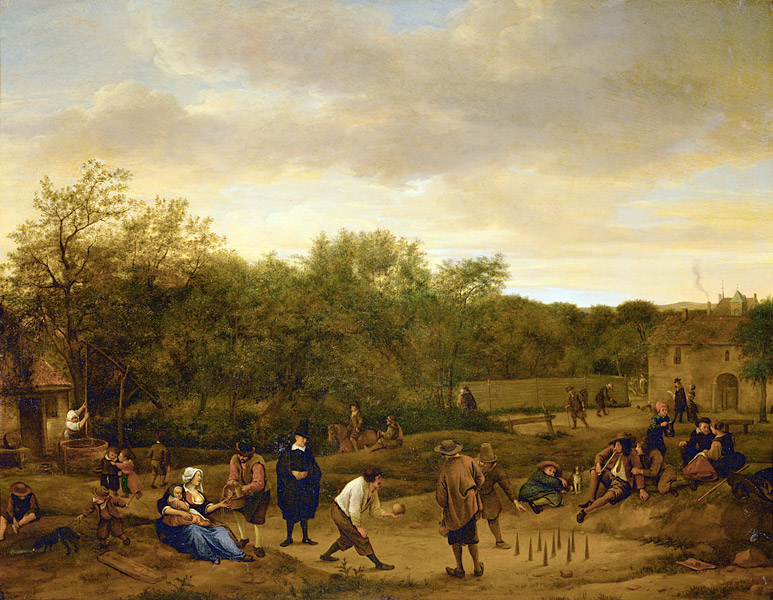
\includegraphics[width=6cm]{French.jpg}
      % \caption{}
    \end{figure}
    \pause
  \end{columns}

\end{frame}

\begin{frame}{概率论的诞生}
\begin{itemize}[<+-|alert@+>]
	\item Cardano虽说是概率的创派始祖, 但概率论真正变成一门学科的标志性事件则是1654年Pascal(帕斯卡)和Fermat(费马)关于两个赌博问题的通信.
	\item Pascal(帕斯卡)就是法国物理学家和数学家帕斯卡, 命名压强单位的物理学家Pascal.
	\item Fermat(费马)就是提出“费马大定理”并且困扰数学家300年之久的费马.
\end{itemize}



\end{frame}




\begin{frame}
  \frametitle{ 两个赌博问题}
  \begin{columns}
    \column{7.5cm}
    \begin{prob}De Mere(德梅尔):事件可能性大小
      \begin{itemize}[<+-|alert@+>]
      \item 一颗骰子投 4 次至少得到一个六点,
      \item 两颗骰子投 24 次至少得到一个双六.
      \end{itemize}
    \end{prob}
    \pause
    \begin{prob}  {\rm De Mere} 分赌注问题
      \begin{itemize}[<+-|alert@+>]
      \item 甲乙两人各下赌注$m$元;
      \item 甲乙两人获胜的概率一样,均为$\frac{1}{2}$;
      \item 先胜$t$局者取得全部赌金;
      \item 甲胜$a$局而乙胜$b$局时赌博被迫中止;
      \item 问赌注如何分?
      \end{itemize}
    \end{prob}
    \column{4cm}
    \vspace{-0.5cm}
    \begin{figure}[htbp]\nonumber


      \centering
      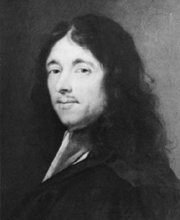
\includegraphics[width=3.5cm]{DeMere.jpg}
      \vspace{0cm}

      \centering{\rm Chevalier De Mere }


      % \caption{}
    \end{figure}
  \end{columns}
\end{frame}
\begin{frame}{骰子点数问题}
\begin{itemize}[<+-|alert@+>]
	\item 据经验所知,一颗骰子投 4 次至少得到一个六点的概率大于$\dfrac{1}{2}$;
	\item 两颗骰子掷一次的结果6倍于一颗骰子掷一次的结果, 则两颗骰子投 24 次至少得到一个双六的概率也应大于$\dfrac{1}{2}$;
	\item 但赌场经验却并非如此.%两颗骰子投 24 次至少得到一个双六的概率小于$\dfrac{1}{2}$;
	\item 考虑成功概率为$p$的随机试验, 连续做$n$次,我们来确定至少一次成功的概率为$q_0$对应的$n$:
	\[1-(1-p)^n=q_0\Rightarrow n=\dfrac{\ln(1-q_0)}{\ln(1-p)}=\dfrac{-\ln(1-q_0)}{p+\frac{p^2}{2}+\cdots}\approx \dfrac{-\ln(1-q_0)}{p};\]
	\item 两个不同成功概率的随机试验, 连续做$n$次, 要保其至少成功一次的概率相同所需要的$n$近似反比于单次试验成功的概率.
\end{itemize}


\end{frame}




\begin{frame}{分赌注问题历史}
	\vspace{-0.15cm}
\begin{itemize}[<+-|alert@+>]
	\item 分赌注问题最早是由意大利数学家Paccioli(帕乔利)在1494年提出, 当时Paccioli给出的答案是按$a:b$进行分配.
	\item 50年后, Tartaglia(塔尔塔利亚)提出反对意见:根据这条规则,如果游戏在一轮之后停止,那么其中一名玩家就会得到全部赌注.
	\item Tartaglia试图修改帕乔利的规则, 以便将上述情况考虑进去, 但最后他怀疑这个问题可能根本没有确定的答案.
	\item 1537年, Cardano也曾经思考过这个问题.
	\begin{itemize}[<+-|alert@+>]
		\item Cardano给出了一个公式$f(n)=1+...+n$, 甲还剩$s-a$局就可以获胜,乙还剩$s-b$局可以获胜, 两者的分金比率应该为$f(s-b):f(s-a)=(s-b)(s-b+1):(s-a)(s-a+1)$.
		%\item 若$s=6,a=5,b=3$, 则上述比为$6:1$.
		\item 虽然Cardano答案错误, 但Cardano已经开始考虑用未来剩余的赌局来决策,而不是局限于已发生的事件.
	\end{itemize}
    \item 直到1654年, De Mere向Pascal请教, Pascal和Fermat进行书信交流, 并且用不同的解法给出了这个问题的正确答案.
    \item 后来, 荷兰数学家Huygens也参与了Pascal和Fermat的讨论, 并在1657年出版书籍《De ratiociniis in ludo aleae ("On Reasoning in Games of Chance")》.

\end{itemize}


\end{frame}


\begin{frame}
  \frametitle{{\rm Blaise Pascal} (布莱士·帕斯卡)}
  \begin{columns}
    \column{4cm}
    % \vspace{2.5cm}
    \begin{figure}[htbp]\nonumber

      \centering
      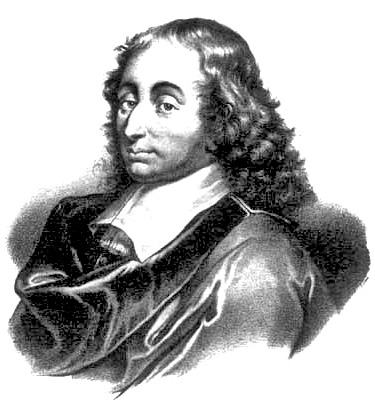
\includegraphics[width=4cm]{pascal1.jpg}

    \end{figure}
    \column{6.5cm}
    \begin{itemize}[<+-|alert@+>]
    \item 16 岁时发现著名的帕斯卡六边形定理:内接于一个二次曲线的六边形的三双对边的交点共线;
    \item 17 岁时写成《圆锥曲线论》,是研究德札尔格射影几何工作心得的论文;
    \item 设计并制作了一台能自动进位的加减法计算装置,被称为是世界上第一台数字计算器;
    \item 以积分学的原理解决了摆线问题;
    \item 与费马相互通信探求赌注分配问题,形成概率论中一个重要的基本概念—数学期望.
    \end{itemize}
  \end{columns}
\end{frame}



\begin{frame}
  \frametitle{{\rm Pierre de Fermat} (皮耶·德·费玛)}
  \begin{columns}
    \column{4cm}
    % \vspace{2.5cm}
    \begin{figure}[htbp]\nonumber

      \centering
      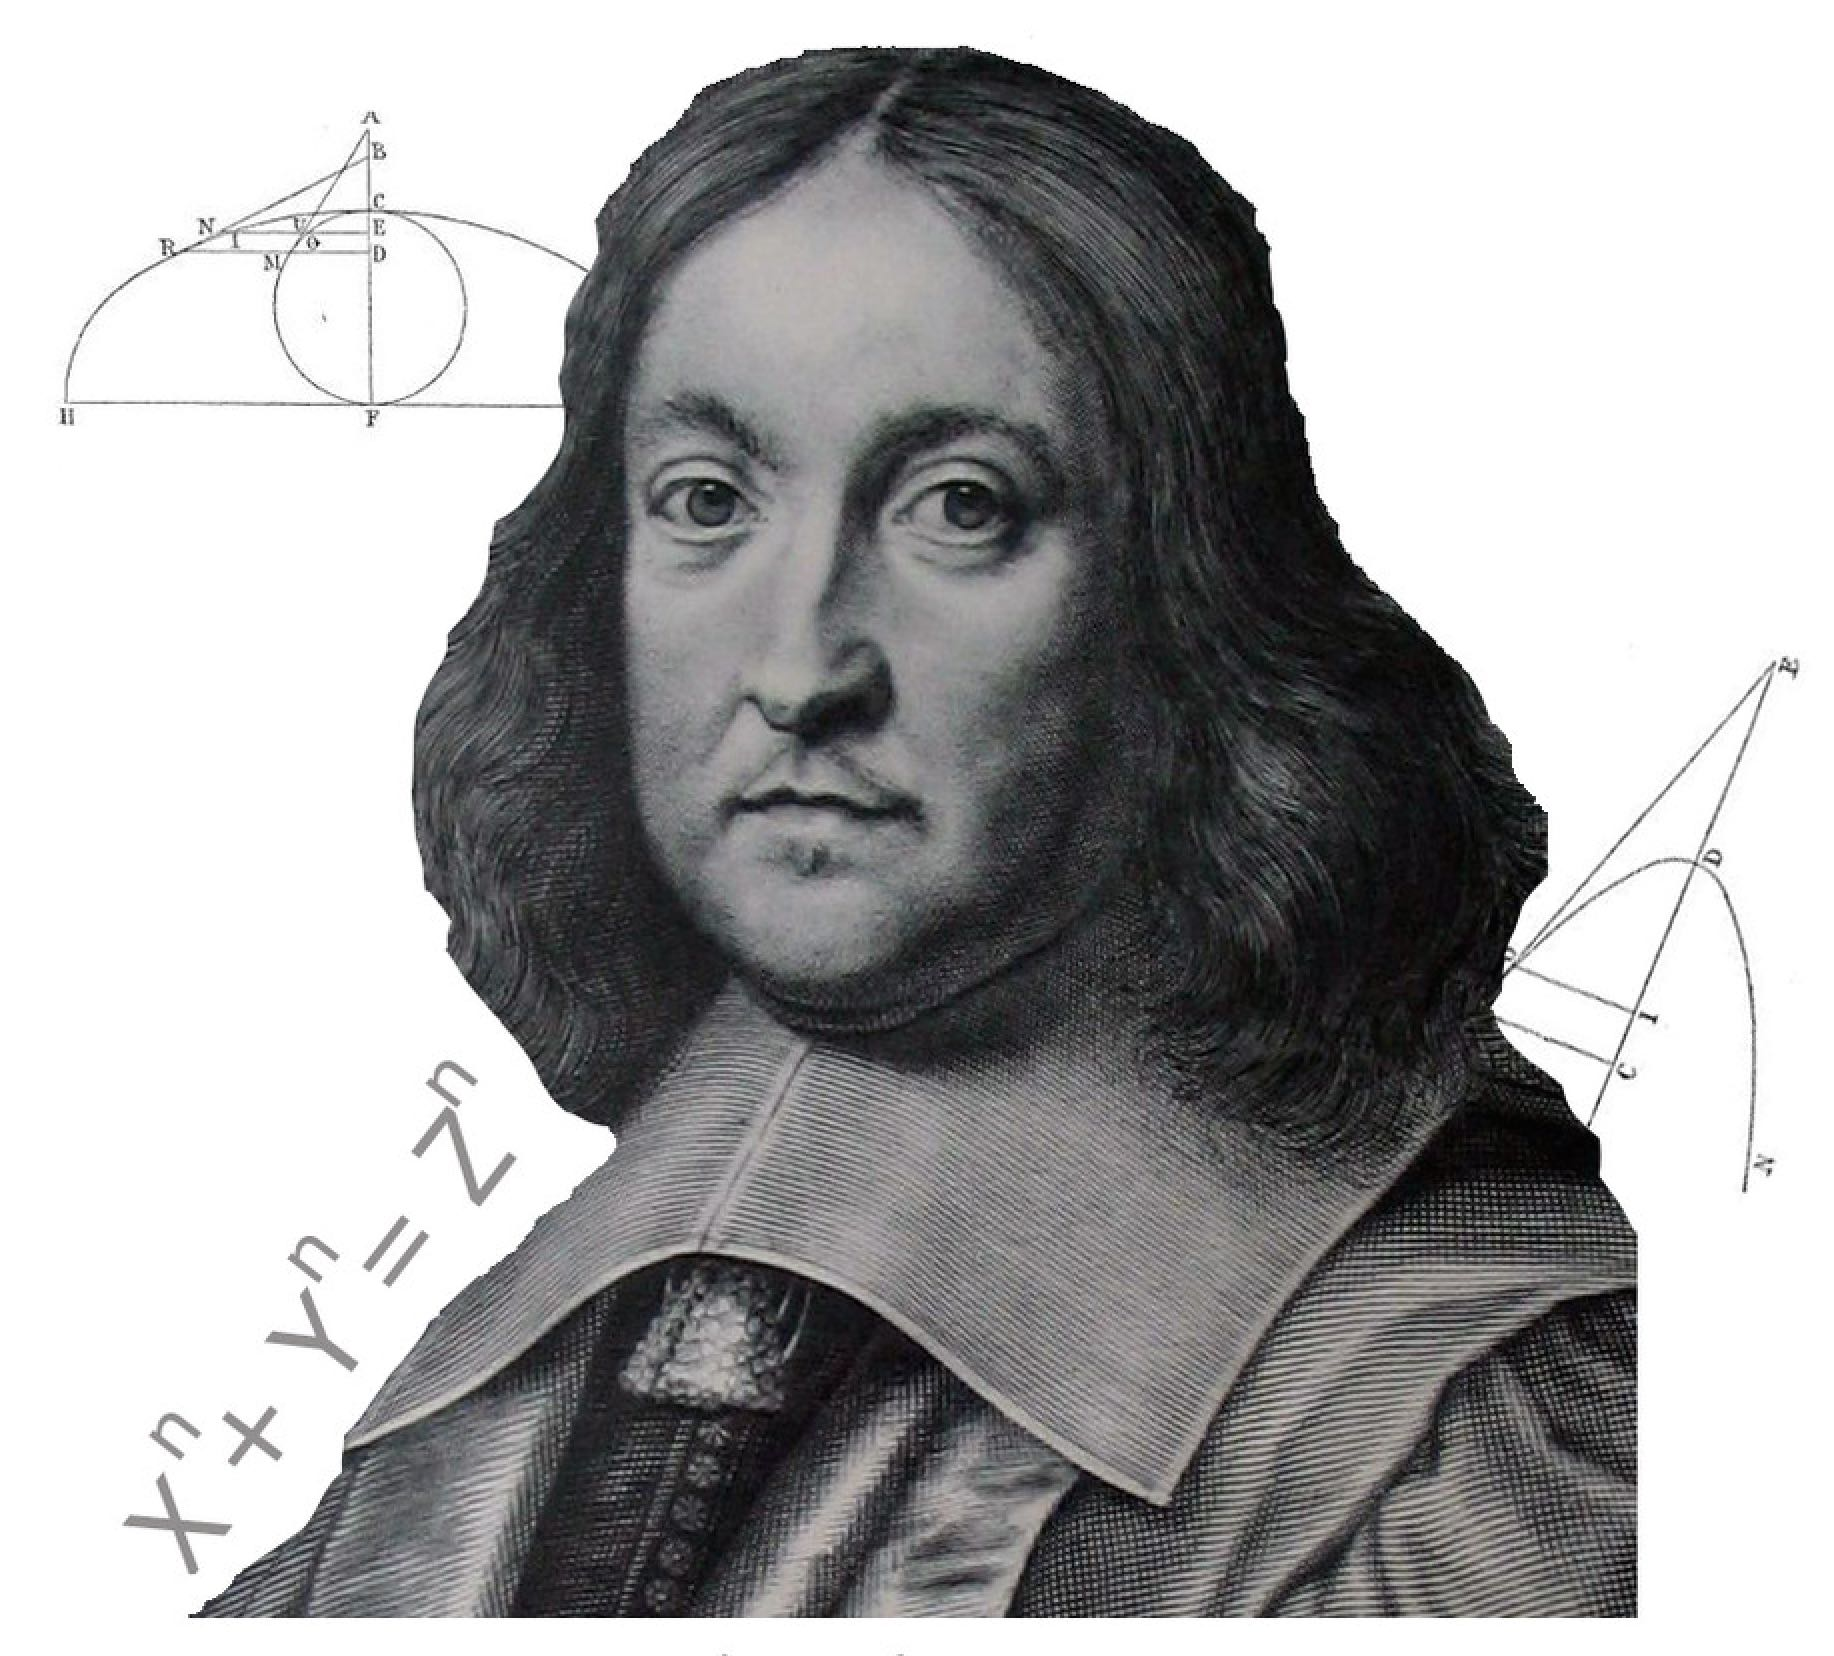
\includegraphics[width=4cm]{Fermat.jpg}

    \end{figure}
    \column{6.5cm}
    \begin{itemize}[<+-|alert@+>]
    \item 独立于笛卡儿发现了解析几何的基本原理;
    \item 求切线、求极大值和极小值以及定积分方法;
    \item 费马和帕斯卡在相互通信探求赌注分配问题,形成概率论中一个重要的基本概念—数学期望;
    \item 数论中的费马大小定理;
    \item 光学的最小作用原理.
    \end{itemize}
  \end{columns}
\end{frame}


\begin{frame}
  \frametitle{{\rm Christiaan Huygens }(克里斯蒂安·惠更斯)}
  \begin{columns}
    \column{6cm}
    \begin{itemize}[<+-|alert@+>]
    \item {\rm Christiaan Huygens} 在 1657 年写了世界上第一本关于概率论的著作 {\rm De ratiociniis in ludo aleae (``On Reasoning in Games of Chance")}, 中文译名``论赌博中的计算”.
    \item 概率论的基本概念、第一次在书中提出期望.
    \end{itemize}

    \column{4cm}
    \begin{figure}[htbp]
      \centering
      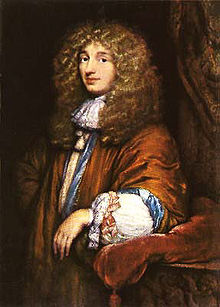
\includegraphics[width=3.5cm]{ChristiaanHuygens.jpg}
    \end{figure}
  \end{columns}
\end{frame}

\begin{frame}{分赌注问题:{\rm Fermat}解法}
\begin{itemize}[<+-|alert@+>]
	\item 显然甲乙距离赢得赌局分别还差$r=t-a$局和$s:=t-b$局. 因此,若赌局不终止,赌局肯定会在接下来的$r+s-1$轮内结束.
	\item 考虑所有$r+s-1$场赌局的结果, 计算在所有可能结果中,甲乙最终获胜的概率. 这样一来,整个问题就简化为一个古典概型的概率计算问题.%关于等概率情况的问题,通过计数就可以算出概率
	\item 以上述计算出来的获胜概率作为分配赌注的比例.
	\item 若$t=6,a=5,b=3$, 则最多还需要赌$3$场就可以分出胜负. 后续所有可能的结果分别为
	$$\{\text{甲甲甲,甲甲乙,甲乙甲,甲乙乙,乙甲甲,乙甲乙, 乙乙甲, 乙乙乙}\}.$$
	\item 所有的$7$种结果中, 乙只有一个结果获胜, 也就是连胜三局, 故赌注分配比例应为$7:1$.
\end{itemize}


\end{frame}

\begin{frame}{分赌注问题:{\rm Pascal}解法}
\begin{itemize}[<+-|alert@+>]
	\item 杨辉三角或Pascal三角法
	\begin{itemize}[<+-|alert@+>]
		\item 后续$r+s-1$场赌局的所有可能结果中:

		使得甲获胜的结果个数为: $n_{\text{甲}}=\sum_{k=r}^{r+s-1}C_{r+s-1}^k$

		使得乙获胜的结果个数为: $n_{\text{乙}}=\sum_{k=s}^{r+s-1}C_{r+s-1}^k$
		\item 若$t=6,a=5,b=3$即$r=1,s=3$, 则
		$$n_{\text{甲}}=C_3^1+C_3^2+C_3^3=7, \quad n_{\text{乙}}=C_3^3=1$$
	\end{itemize}


\end{itemize}

\end{frame}


\begin{frame}{分赌注问题:{\rm Pascal}解法}
	\begin{itemize}[<+-|alert@+>]
		\item 递推法
		\begin{itemize}[<+-|alert@+>]
			\item 假设甲和乙赌注共$64$个金币, 考虑$t=6,a=5,b=4$的情况:

			如果下一局甲胜,则甲得到全部64枚金币

			如果下一局甲输,则比分变为$5:5$, 这时候是平局,甲乙平分赌注.

			\item 不管哪种情况, 甲至少会拿$32$个金币,剩余的$32$个金币,可能归甲也可能归乙,平分. 这样甲应该拿$32+(64-32)/2=48$个金币,乙则拿$16$个金币.
			\item 考虑$t=6,a=5,b=3$的情况:
			\begin{itemize}[<+-|alert@+>]
				\item 如果下一局甲胜,则拿到所有赌注;
				\item 如果甲败,则问题转化为$t=6,a=5,b=4$的情况;
				\item 由此可见,甲至少可拿48个硬币,剩余金币平分;
				\item 因此,甲最终可拿$48+(64-48)/2=56$个金币, 乙拿8个金币;
				\item 和Fermat的$7:1$结果相同.
			\end{itemize}


			%\item Pascal分析了一个简化版本, 就是$t=3,a=2,b=1$的情况.
			%\item 假设甲和乙的赌注一共为$64$个金币, 当$2:1$比分的情况下:

			%%如果甲输了,则比分变成$2:2$,这时候是平局,甲乙平分奖金.

			%\item 不管哪一种情况, 甲至少会拿$32$个金币,至于剩余的$32$个金币,可能归甲也可能归乙,平分. 这样甲应该拿$32+(64-32)/2=48$个金币,乙则拿$16$个金币.

			%\item 考虑$t=6,a=5,b=4$的情况: 与$t=3,a=2,b=1$的情况类似, 甲应该拿$32+(64-32)/2=48$个金币.
		\item 在递推解法里,Pascal用到了期望的思想,尤其是$48+(64-48)/2$这个式子.
		\begin{itemize}[<+-|alert@+>]
			\item 下一局甲胜得到$x=64$个金币,甲输得到$y=48$个金币;
			\item 按Pascal的式子, 甲拿到的金币为: $y+(x-y)/2=(x+y)/2=x*0.5+y*0.5$,这其实就是条件期望公式.
		\end{itemize}

		\end{itemize}

	\end{itemize}

	\end{frame}

\begin{frame}{分赌注问题:{\rm Pascal}递推法的一般解法}
\begin{itemize}[<+-|alert@+>]
	\item 赌博中断时,甲乙距离赢得赌局分别还差$r=t-a$局和$s:=t-b$局;
	\item 假设中断后赌局继续进行, 甲最终获胜的概率记为$e(r,s)$, 则有边界条件:
	\[e(0,s)=1,\quad e(r,0)=0,\quad e(r,r)=1/2\]且有如下递推式
	\[e(r,s)=[e(r-1,s)+e(r,s-1)]/2.\]
	\item 上式用到了全概率公式,是一个偏差分方程. Pascal借助算术三角阵, 利用数学归纳法得到
	\[
	e(r, s)=\frac{D_{r+s-1, s-1}}{D_{r+s-1}} (r+s=2,3, \cdots)
	\]
	\item 这里分子表示算术三角形中第${r+s-1}$行最后${s}$项之和,而分母为第${r+s-1}$行的所有数字之和, 故为${2^{r+s-1}}$.
\end{itemize}


\end{frame}





\begin{frame}
  \frametitle{{\rm Jacob Bernoulli}(雅各布·伯努利)}
  \begin{columns}
    \column{6cm}
    \begin{itemize}[<+-|alert@+>]
    \item 概率论与变分法先驱之一;
    \item 第一次使用``积分"一词;
    \item 首次给出直角坐标和极坐标下的曲率半径公式;
    \item 1713 年出版 《Ars Conjectandi》(可译为《猜度术》):提出了概率论中的“伯努利大数定律” - 大数定律的最早形式.
    \end{itemize}

    \column{5cm}

    \begin{figure}[htbp]
      \centering
      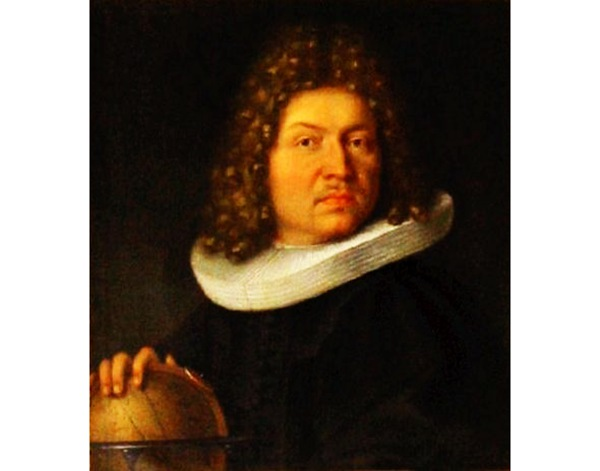
\includegraphics[width=5.5cm]{Bernoulli.jpg}
    \end{figure}
  \end{columns}
\end{frame}



\begin{frame}
  \frametitle{{\rm Abraham de Moivre}(亚伯拉罕·棣莫弗)}
  \vspace{-0.15cm}
  \begin{columns}
    \column{6.5cm}
    \begin{itemize}[<+-|alert@+>]
    \item 棣莫弗公式:$$(\cos x+i\sin x)^n=\cos(nx)+i \sin(nx)$$

    \item 二项分布的正态逼近:棣莫弗-拉普拉斯中心极限定理;
    \item 利用概率生成函数计算均匀分布随机变量和的分布;
    \item 寿险保险数学:年金的分析与计算.
    \item 开创了概率论的现代方法:1718 年发表了《The Doctrine of Chance》. 在此书中
	统计独立性的定义首次出现. 该书在 1738 年与 1756 年出了扩展版,生日问
	题出现在 1738 年的版本中,赌徒破产问题出现在 1756 年的版本中.
    \end{itemize}

    \column{5cm}

    \begin{figure}[htbp]
      \centering
      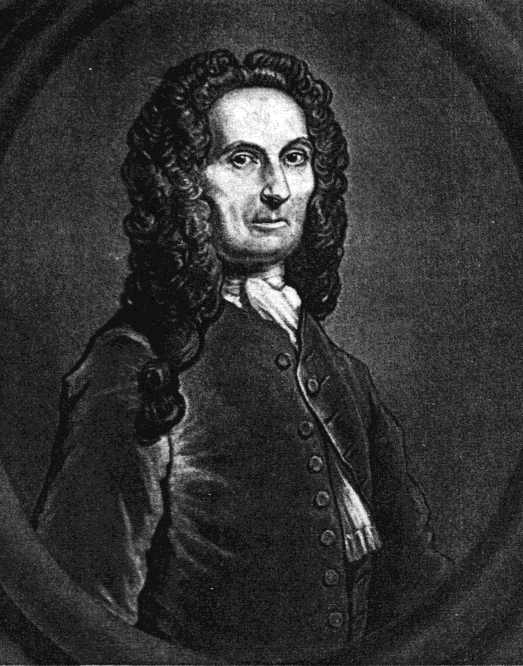
\includegraphics[width=4.5cm]{deMoivre.jpg}
    \end{figure}
  \end{columns}
\end{frame}












\begin{frame}
  \frametitle{{\rm Pierre-Simon Laplace}(皮埃尔-西蒙·拉普拉斯)}
  \begin{columns}
    \column{6cm}
    \begin{itemize}[<+-|alert@+>]
    \item {\rm Pierre-Simon Laplace} 在他 1812 年的著作{\rm 《Th{\'e}orie Analytique des Probabilit{\`i}{\'e}s》}(可
	译为《概率论的解析理论》)中介绍了概率的数学理论及其科学应用;

    \item {\rm Laplace}只考虑了古典概型, 对一般的概率及其应用没有介绍;
    \item 到 1850 年, 许多数学家发现古典概型对一般场合不合理, 开始尝试重新定义概率.
    \end{itemize}

    \column{5cm}

    \begin{figure}[htbp]
      \centering
      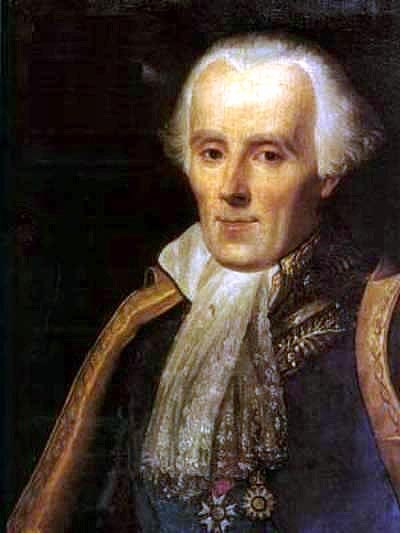
\includegraphics[width=4.5cm]{Laplace.jpg}
    \end{figure}
  \end{columns}
\end{frame}




\begin{frame}{概率的公理化体系}

\begin{itemize}[<+-|alert@+>]
    \item  从 17 世纪到 19 世纪长达 300 多年的时间里,以 Laplace(1749 一
1827), De Moivre(1687-1754), J.Bernouil, D.Bernouli(1700--1782).
Pascal、Fermat 等为代表的优秀学者从各自不同的角度对概率论的许多方面进行了深入细致的研究,取得了大量成果,可是都无法将概率论纳入到严格的公理化体系中.而概率论作为数学的重要分支,其逻辑的严密性和完整性始终受到质疑.
\item 数学大师 Hilbert(1862—1943)在 1900 年提出的 23 个著名问题中,第 6 个问题是关于“物理定律的公理化”,其中就涉及概率论的公理化问题.
\item 激发了以 Borel(1871 一 1956)和 Lebesgue(1875—1941)等为代表的一批学者的研究热情.他们在测度理论(Measure Theory)方面得到的成果为后续研究指明了道路.
\end{itemize}
\end{frame}





\begin{frame}
  \frametitle{{\rm Andrey Kolmogorov}(安德列·柯尔莫哥洛夫)}
  \begin{columns}
    \column{6cm}
    \begin{itemize}[<+-|alert@+>]
    \item {\rm Andrey Kolmogorov} 第一个在他 1933 年的著作{\rm 《Grundbegriffe der Wahrscheinlichkeitsrechnun》(《Foundations of the Theory of Probability》)} 中严格的定义了概率;
    \item 类似于{\rm Euclid}基于公理体系建立几何, 他从基本公理建立了概率理论, 从而使概率论称为一门严谨的数学分支;
    \item 概率理论的现代研究和测度论非常紧密的结合在一起.

    \end{itemize}

    \column{5cm}

    \begin{figure}[htbp]\nonumber
      \centering
      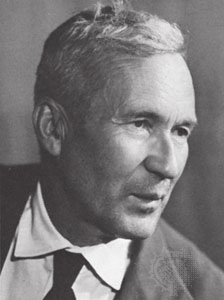
\includegraphics[width=4cm]{Kolmogorov.jpg}

      \centering{\rm 1903.4.25-1987.10.20}

    \end{figure}
  \end{columns}
\end{frame}
\begin{frame}
  \frametitle{{\rm Kolmogorov} 成就}
  \vspace{-0.4cm}
  {\small\begin{itemize}[<+-|alert@+>]
    \item 20 世纪最伟大的数学家之一,在概率论、实分析、拓扑学、泛函分析、微分方程、生物数学、等很多领域都有着开创性的贡献.

    \item 1933 年,出版《概率论基础》,首次将概率论建立在严格的公理基础上,解决了希尔伯特第 6 问题的概率部分。
    \item 线性拓扑空间理论的创始人之一, 和美国著名数学家亚历山大({\rm J.W.Alexander})同时独立引入上同调群的概念;

    \item 40 年代, 在遗传学、弹道学、气象学、金属结晶学等有重要贡献;
    \item 50 年代, 经典力学、遍历理论、函数论、信息论、算法理论等。

    \item 柯尔莫哥洛夫的研究几乎遍及数论之外的一切数学领域。1963 年,在第比利斯召开的概率统计会议上,美国统计学家沃尔夫维茨({\rm J.Wolfowitz})说:``我来苏联的一个特别的目的是确定柯尔莫哥洛夫到底是一个人呢,还是一个研究机构.”


    \end{itemize}}
\end{frame}

\begin{frame}
  \frametitle{{\rm Kolmogorov} 轶事}
  \begin{itemize}[<+-|alert@+>]
  \item  历史学要证实自己的观点需要几个甚至几十个正确证明才行,数学只需要一个证明就行, 于是转行数学.
  \item 20 年代的莫斯科大学,学生被要求在十四个不同的数学分支参加十四门考试;但考试可用相应领域的独立研究代替. {\rm Kolmogorov} 从来没有参加考试,他写了十四个不同方向的有新意的文章。
  \item {\rm Kolmogorov}总是以感激的口气提到斯大林:“首先,他在战争年代为每一位院士提供了一床毛毯;第二,原谅了我在科学院的那次打架。”{\rm Kolmogorov}一次在选举会上打了{\rm Luzin}(卢津)一个耳光,他说:“(打架)那是我们常用的方式。”{\rm Luzin}在实变函数方面有着很重要的贡献,但是以打架而论,远非{\rm Kolmogorov}的对手.
  \end{itemize}
\end{frame}


